\section{Reference Diagnostic and Prognostic Model Reproduction}
\label{sec:reference}

\subsection{Purpose and evidence boundary}
\label{sec:reference:scope}

The reference workflow supplies the conventional statistical baseline for the
project: logistic regression for liver metastasis at diagnosis and Cox regression
for overall survival within the liver-positive cohort. The workflow of
\citet{Li2023} is reconstructed using the cohorts in Section~\ref{sec:data} so that
subsequent TabPFN transformations, foundation-model comparisons, nonlinear heads
and augmentation experiments can be interpreted against a transparent clinical
reference.

This is a methodological reproduction rather than a patient-identical replication.
The SEER release used by the article was no longer the available project source, so
the preprocessing pipeline constructed a clinically similar cohort from the
available SEER export. The article's external hospital cohort was also unavailable.
Accordingly, agreement in selected variables or performance is informative, but a
difference does not by itself indicate a reproduction failure or a model improvement.

The two tasks follow different evaluation designs from the reference study. For
diagnosis, the complete SEER cohort is used to develop the models and to calculate
ROC/AUC, calibration and decision curves. The reference article likewise calls its
complete SEER diagnostic cohort the training cohort and evaluates it separately
from its external hospital cohort. For prognosis, the liver-positive SEER cohort
is divided into a 70\% training subset and a 30\% internal-validation subset.
Diagnostic results therefore describe performance in the same cohort used for
model development, whereas the prognostic results include evaluation in patients
held out from model fitting. This distinction is stated whenever the two tasks are
compared.

\subsection{Candidate descriptors and task-specific designs}
\label{sec:reference:candidates}

Both reproductions begin from the same 17 clinical descriptor families
(Table~\ref{tab:reference:candidates}), after the preprocessing and complete-case
rules in Section~\ref{sec:data}. The task datasets differ in their target and
eligible population: diagnosis uses the full cohort and predicts liver metastasis
at diagnosis, whereas prognosis is restricted to patients already recorded with
liver metastasis and predicts overall survival. Both histology definitions follow
the reference study. The diagnostic analysis retains the individual ICD-O
histological subtypes available in the cohort (10 categories), whereas the
prognostic analysis applies the paper's coarser 2-group definition: carcinoid
tumour NOS and atypical carcinoid tumour versus all other listed histological
subtypes.

\begin{table}[htbp]
\centering\small
\caption{Overview of the two reference-reproduction tasks. Evaluation procedures
are described in detail in the task-specific subsections.}
\label{tab:reference:task_overview}
\begin{tabularx}{\linewidth}{@{}p{0.15\linewidth}p{0.27\linewidth}p{0.25\linewidth}Y@{}}
\toprule
Task & Population and outcome & Development design & Principal evaluation \\
\midrule
Diagnosis & 2,672 patients; 462 liver-metastasis cases (17.3\%) & Complete SEER
cohort used for model development and within-cohort evaluation & ROC/AUC, Brier score, calibration and
decision curves \\
Prognosis & 462 liver-positive patients; overall survival and death indicator &
323-record training subset and 139-record internal-validation subset & Harrell
C-index, time-dependent AUC, calibration, decision curves and Kaplan--Meier
(K--M) survival curves \\
\bottomrule
\end{tabularx}
\end{table}
\FloatBarrier

\begingroup
\small
\setlength{\LTpre}{0.3em}
\setlength{\LTpost}{0.5em}
\begin{longtable}{@{}p{0.27\linewidth}p{0.18\linewidth}p{0.47\linewidth}@{}}
\caption{17 candidate clinical descriptor families entering the reference
feature-selection workflows.}\label{tab:reference:candidates}\\
\toprule
Descriptor & Representation & Modelling description \\
\midrule
\endfirsthead
\multicolumn{3}{@{}l}{\small\itshape Table~\thetable\ continued}\\
\toprule
Descriptor & Representation & Modelling description \\
\midrule
\endhead
\midrule
\multicolumn{3}{r}{\small\itshape Continued on next page}\\
\endfoot
\bottomrule
\endlastfoot
Age at diagnosis & Continuous & Age in years at diagnosis \\
Race & Categorical & SEER race category after preprocessing harmonisation \\
Sex & Binary & Female or male indicator \\
Marital status & Binary & Married versus the harmonised non-married category \\
Histological subtype & Categorical & Both definitions follow the reference study:
diagnosis retains the 10 subtype categories observed in this cohort; prognosis
groups carcinoid and atypical carcinoid tumours together and places the other
subtypes in an ``Others'' category \\
Tumour grade & Ordered categorical & Grade I--IV after the documented SEER mapping \\
Primary-site group & Categorical & Pancreatic head, body, tail or other site group \\
AJCC T stage & Ordered categorical & Harmonised T-stage category \\
AJCC N stage & Binary & N0 versus node-positive disease \\
Primary-site surgery & Binary & Recorded surgery of the primary tumour \\
Lymph-node surgery & Binary & Recorded regional lymph-node surgery \\
Radiotherapy & Binary & Recorded radiotherapy indicator \\
Chemotherapy & Binary & Recorded chemotherapy indicator \\
Tumour-size group & Ordered categorical & $\leq26$ mm, 26--36 mm or $>36$ mm \\
Bone metastasis & Binary & Bone metastasis recorded at diagnosis \\
Brain metastasis & Binary & Brain metastasis recorded at diagnosis \\
Lung metastasis & Binary & Lung metastasis recorded at diagnosis \\
\end{longtable}
\endgroup

General M stage is not included as a diagnostic predictor because it incorporates
distant metastatic disease and would be too closely related to the liver-metastasis
target. Treatment variables are retained to reproduce the reference workflow, but
their temporal availability at a true diagnosis-time prediction point is uncertain.
They must therefore be interpreted as retrospective predictors rather than as
prospectively established decision-time inputs.

\subsection{Diagnostic workflow and selected variables}
\label{sec:reference:diagnostic_methods}

The diagnostic analysis uses all 2,672 retained records, including 462 with liver
metastasis, and 17 candidate clinical predictors. In accordance with the reference
study, tumour size is entered as 3 categories ($\leq26$ mm, 26--36 mm and
$>36$ mm), and N stage is entered once as N0 versus N1. The corresponding
continuous tumour-size field and alternative N-stage encoding are not added as
extra predictors. General M stage is excluded because it directly incorporates
distant metastatic disease and would reveal information closely related to the
liver-metastasis outcome. Treatment variables are retained to reproduce the
reference model, although the SEER records do not establish whether every
treatment was known at the intended prediction time.

The screening sequence starts with 10-fold cross-validated binomial LASSO. The
implemented primary rule uses the one-standard-error penalty to obtain a smaller
set of predictors, while the minimum-deviance penalty is retained as a sensitivity
analysis. Nonzero encoded columns are then mapped back to their clinical
descriptors. This differs slightly from the reference article's LASSO figure,
which identifies the minimum-error penalty \citep{Li2023}.

As in the reference study, a 1,000-tree random forest provides a second view of
predictor importance. Mean decrease in accuracy measures how much predictive
accuracy is lost when a variable is permuted, whereas mean decrease in Gini
summarises how much that variable reduces node impurity across the forest. These
measures rank predictors in different ways; they do not by themselves confirm a
clinical effect or establish causality. The reference article reports a
7-variable random-forest shortlist whose variables were also selected by LASSO.
In this reproduction, the forest ranking is reported alongside LASSO but is not
used as a mandatory filter. The final
data-driven logistic model retains variables from the LASSO shortlist whose global
likelihood-ratio-test has $p<0.05$ in the joint multivariable model. These
screening $p$-values are nominal and are not adjusted for the preceding selection.

The fitted penalties are $\lambda_{\min}=0.0034$ and
$\lambda_{\mathrm{1se}}=0.0182$ at the displayed precision. As shown in
Figure~\ref{fig:reference:lasso}, the one-standard-error rule deliberately accepts
a small increase in cross-validated error in exchange for a sparser model. Because
categorical descriptors expand into multiple design columns, selection is first
performed at the encoded-column level and then mapped back to the originating
clinical descriptor.

\begin{figure}[htbp]
\centering
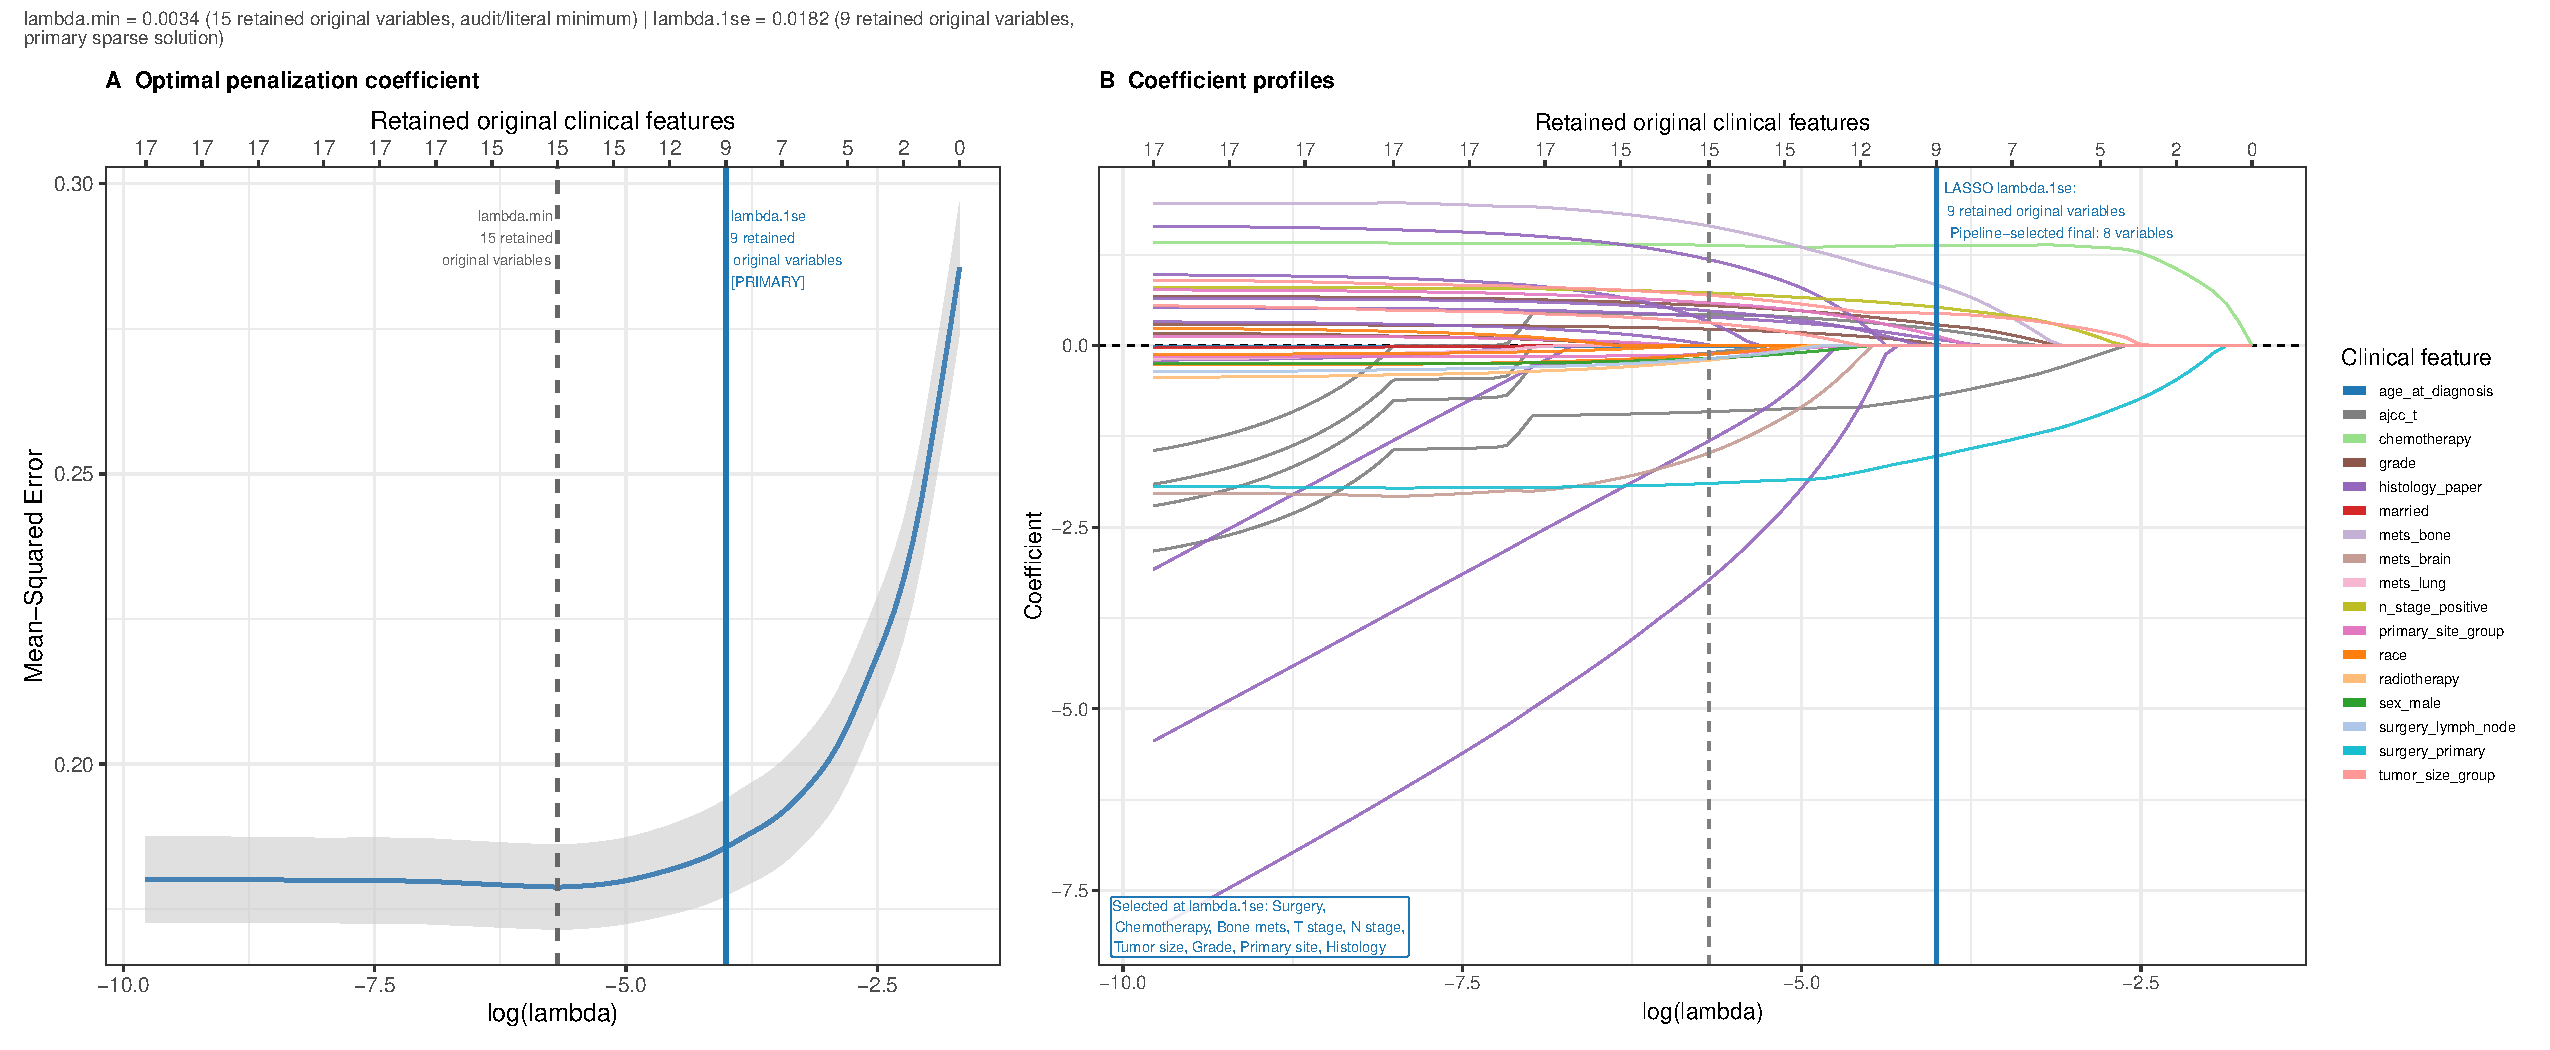
\includegraphics[width=\linewidth]{reference_reproduction/diagnostic_lasso_selection.pdf}
\caption{Diagnostic LASSO feature selection. A: ten-fold cross-validated binomial
error with the minimum-error and one-standard-error penalties. B: coefficient
shrinkage paths for the encoded predictor columns. The top axes count retained
original clinical descriptor families after back-mapping; the primary
$\lambda_{\mathrm{1se}}$ solution retains 9 families, whereas
$\lambda_{\min}$ retains 15. The data-driven final model contains 8 variables
after the subsequent multivariable screen.}
\label{fig:reference:lasso}
\end{figure}

The selection results contain 15 clinical variables at
$\lambda_{\min}$ and 9 at $\lambda_{\mathrm{1se}}$. A total of 8 survive the
multivariable screen: primary-site surgery, chemotherapy, bone metastasis,
T stage, N stage, tumour-size group, primary site and histology. Grade is included
in the 9-variable fit but does not meet the final threshold
($p=0.07306$). This is a result of this particular adjustment and selection
procedure, not evidence that grade is generally uninformative.

Two fixed reference sets are also fitted. The 5-variable
\emph{nomogram-figure} set contains grade, N stage, surgery, tumour size and bone
metastasis; the 6-variable \emph{text-defined} set additionally contains
chemotherapy. Keeping both makes the reference article's text/figure discrepancy
explicit \citep{Li2023}. The data-driven 8-variable model is a separate
reproduction variant, not a relabelling of the published nomogram. The comparator
contains only T stage and N stage and is therefore described as T/N rather than as
a complete TNM-stage model.

Figure~\ref{fig:reference:rf} also cautions against a single feature-importance
interpretation. Chemotherapy and primary surgery rank 1st and 2nd by mean
decrease in accuracy. Age ranks 2nd by Gini decrease but 16th by
permutation importance, with a negative latter value. Thus, the two importance
definitions do not consistently corroborate the same ranking. This discrepancy
supports treating importance as a model-dependent descriptive quantity; it does
not by itself establish confounding or a causal mechanism.

\begin{figure}[htbp]
\centering
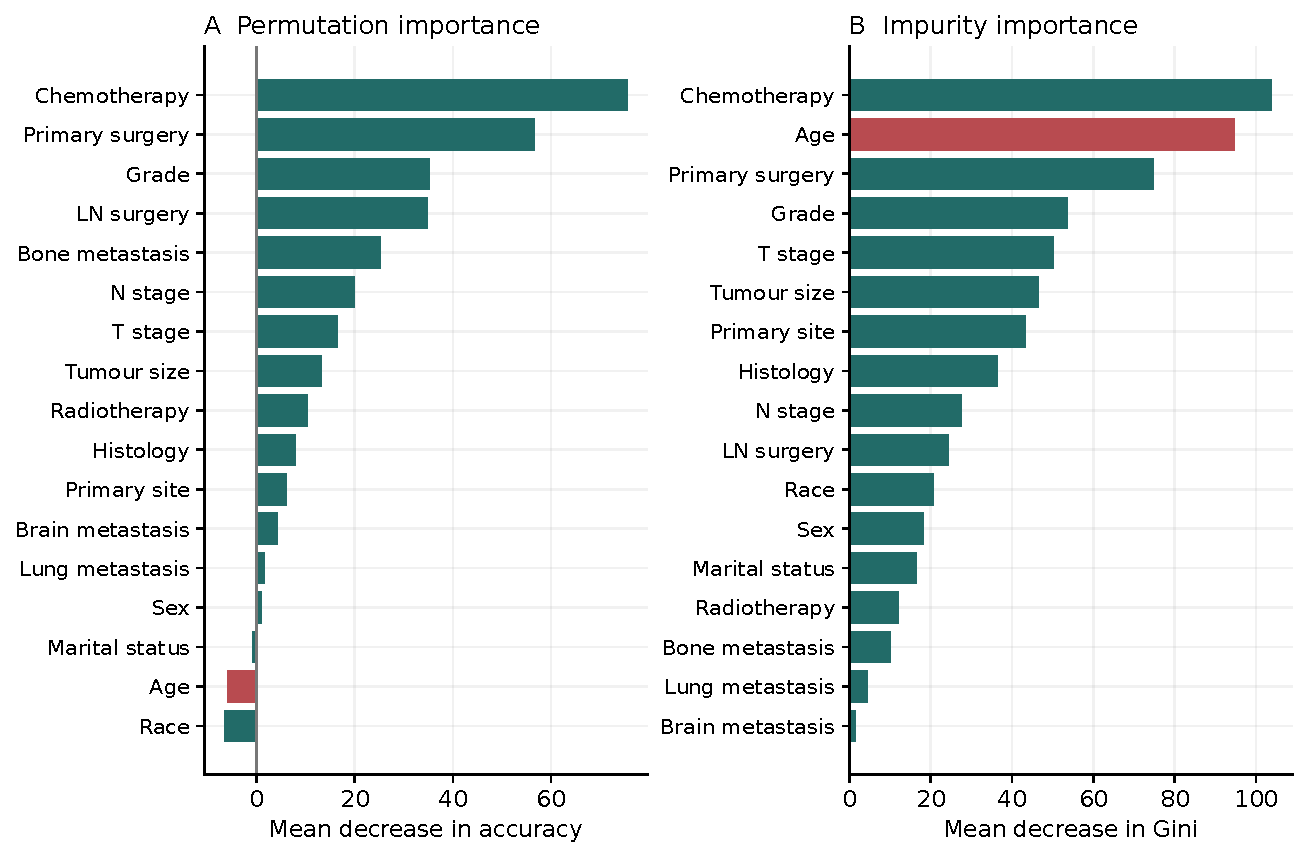
\includegraphics[width=0.82\linewidth]{reference_reproduction/diagnostic_rf_importance.pdf}
\caption{Diagnostic random-forest importance. Panels rank variables independently
under their own criterion; the
highlighted age row makes the disagreement visible. The horizontal scales measure
different quantities and are not directly comparable. These are single-fit
importance estimates, without ranking-stability intervals.}
\label{fig:reference:rf}
\end{figure}
\FloatBarrier

Table~\ref{tab:reference:diagnostic_selection} separates the data-driven selection
path from the fixed reference specifications. This distinction is important: the
5- and 6-variable models ask how the published variable sets behave in the
available cohort, whereas the 8-variable model asks what this cohort's
implemented screening pipeline selects.

\begin{table}[htbp]
\centering\footnotesize
\caption{Diagnostic feature-selection path and evaluated specifications. The
random forest provides an additional importance ranking but does not independently
determine the final feature set.}
\label{tab:reference:diagnostic_selection}
\begin{tabularx}{\linewidth}{@{}p{0.21\linewidth}p{0.27\linewidth}Y@{}}
\toprule
Stage or model & Rule and role & Clinical variables retained or specified \\
\midrule
LASSO, $\lambda_{\min}$ & Minimum cross-validated deviance; sensitivity shortlist &
15 of 17 candidates: all except marital status and lung metastasis \\
LASSO, $\lambda_{\mathrm{1se}}$ & Primary sparse shortlist &
Primary surgery, chemotherapy, bone metastasis, T stage, N stage, tumour size,
grade, primary site and histology \\
Pipeline-selected final & Global likelihood-ratio-test $p<0.05$ within the
9-variable shortlist & Primary surgery, chemotherapy, bone metastasis, T stage,
N stage, tumour size, primary site and histology; grade is excluded ($p=0.0731$) \\
Paper-text model & Fixed 6-variable reference set & Grade, N stage, primary
surgery, chemotherapy, tumour size and bone metastasis \\
Nomogram-figure model & Fixed 5-variable primary reproduction target & Grade,
N stage, primary surgery, tumour size and bone metastasis \\
T/N baseline & Conventional comparator & T stage and N stage \\
\bottomrule
\end{tabularx}
\end{table}

The second-stage screen is shown variable by variable in
Table~\ref{tab:reference:diagnostic_screen}. The reported likelihood-ratio-test
$p$-values are global tests for each clinical descriptor in the joint
9-variable logistic model. They are used to reproduce the implemented selection
rule and should not be interpreted as multiplicity-adjusted confirmatory inference.

\begin{table}[htbp]
\centering\small
\caption{Diagnostic multivariable screen applied to the 9
$\lambda_{\mathrm{1se}}$ clinical descriptors.}
\label{tab:reference:diagnostic_screen}
\begin{tabularx}{0.78\linewidth}{@{}Yrr@{}}
\toprule
Clinical descriptor & Global nominal $p$ & Final status \\
\midrule
\csname @@input\endcsname{tables/reference_reproduction/diagnostic_multivariable_screen_rows.tex}
\bottomrule
\end{tabularx}
\end{table}

\FloatBarrier

\subsection{Diagnostic model evaluation and results}
\label{sec:reference:diagnostic_results}

\paragraph{Evaluation protocol.}
The reference article uses the complete SEER diagnostic cohort as its training
cohort; it does not describe a separate internal hold-out set for the diagnostic
model. Its 70/30 internal split applies to the prognostic analysis. The reproduction
therefore follows the diagnostic design by fitting and evaluating all 4 logistic
specifications in the complete 2,672-patient SEER cohort. Discrimination is
summarised by ROC curves and AUC with a requested 1,000-resample interval.
Calibration is assessed using the Brier score and calibration intercept/slope for
the 5-variable primary model; the pipeline-selected model additionally has an
uncorrected curve and a bootstrap-corrected calibration curve. Decision-curve
analysis compares model net benefit with T/N, treat-all and treat-none strategies
across threshold probabilities. Because the diagnostic models are evaluated in the
same records used for fitting, these results may overestimate performance in new
patients and are not equivalent to held-out or external validation.

\paragraph{Discrimination.}
Table~\ref{tab:reference:diagnostic_auc} gives the AUC estimates in the complete
2,672-record diagnostic development cohort. The pipeline-selected model has the
largest AUC, 0.9028, followed by 0.8947 for the paper-text model, 0.8795 for the
nomogram-figure model and 0.7628 for T/N. The reference article reports a SEER
training-cohort AUC of 0.877 and an external-hospital AUC of 0.893 \citep{Li2023}. The
proximity of the published internal estimate to 0.8795 is descriptive agreement
across different extracts, not a test of reproduction fidelity or model equivalence.

\begin{table}[htbp]
\centering\small
\caption{Diagnostic discrimination in the complete SEER development cohort
($n=2,672$), following the reference study's diagnostic training-cohort design.
Each model is fitted and evaluated in these same records; brackets show 95\% AUC
intervals and not held-out performance intervals.}
\label{tab:reference:diagnostic_auc}
\begin{tabularx}{\linewidth}{@{}Ycr@{}}
\toprule
Model & Clinical variables & Within-cohort AUC [95\% interval] \\
\midrule
\csname @@input\endcsname{tables/reference_reproduction/diagnostic_auc_rows.tex}
\bottomrule
\end{tabularx}
\end{table}

The AUC routine requests 1,000 bootstrap resamples of the outcome--prediction
pairs. It does not repeat feature selection or model fitting inside those
resamples. If that calculation fails, the routine uses a DeLong interval, although
the result table does not identify which method supplied each interval. These
intervals therefore quantify uncertainty around the reported AUCs but are not
whole-pipeline bootstrap validation. The internal LASSO cross-validation selects
the penalty; it does not turn the final full-cohort AUC into a held-out estimate.

For the 5-variable primary model, the within-cohort Brier score is 0.0969.
The fitted calibration intercept and slope round to 0 and 1 on the training data.
Such values are expected for an unpenalised logistic model evaluated on its own
fitting sample and do not establish transportable calibration. The separate
pipeline-selected calibration curve includes a bootstrap correction conditional
on its already selected variable set (Figure~\ref{fig:reference:diagnostic_eval}B).
That procedure does not account for reselecting the variables.

The diagnostic decision curves in Figure~\ref{fig:reference:diagnostic_eval}C
compare the pipeline-selected model, T/N and the two default strategies. They
describe net benefit in the same cohort used for model fitting. No clinical action or acceptable
threshold range was prospectively defined here, and treatment-related inputs
have not been shown to precede prediction. The curves therefore cannot establish
a deployable diagnostic intervention or benefit in a new hospital.

\begin{figure}[htbp]
\centering
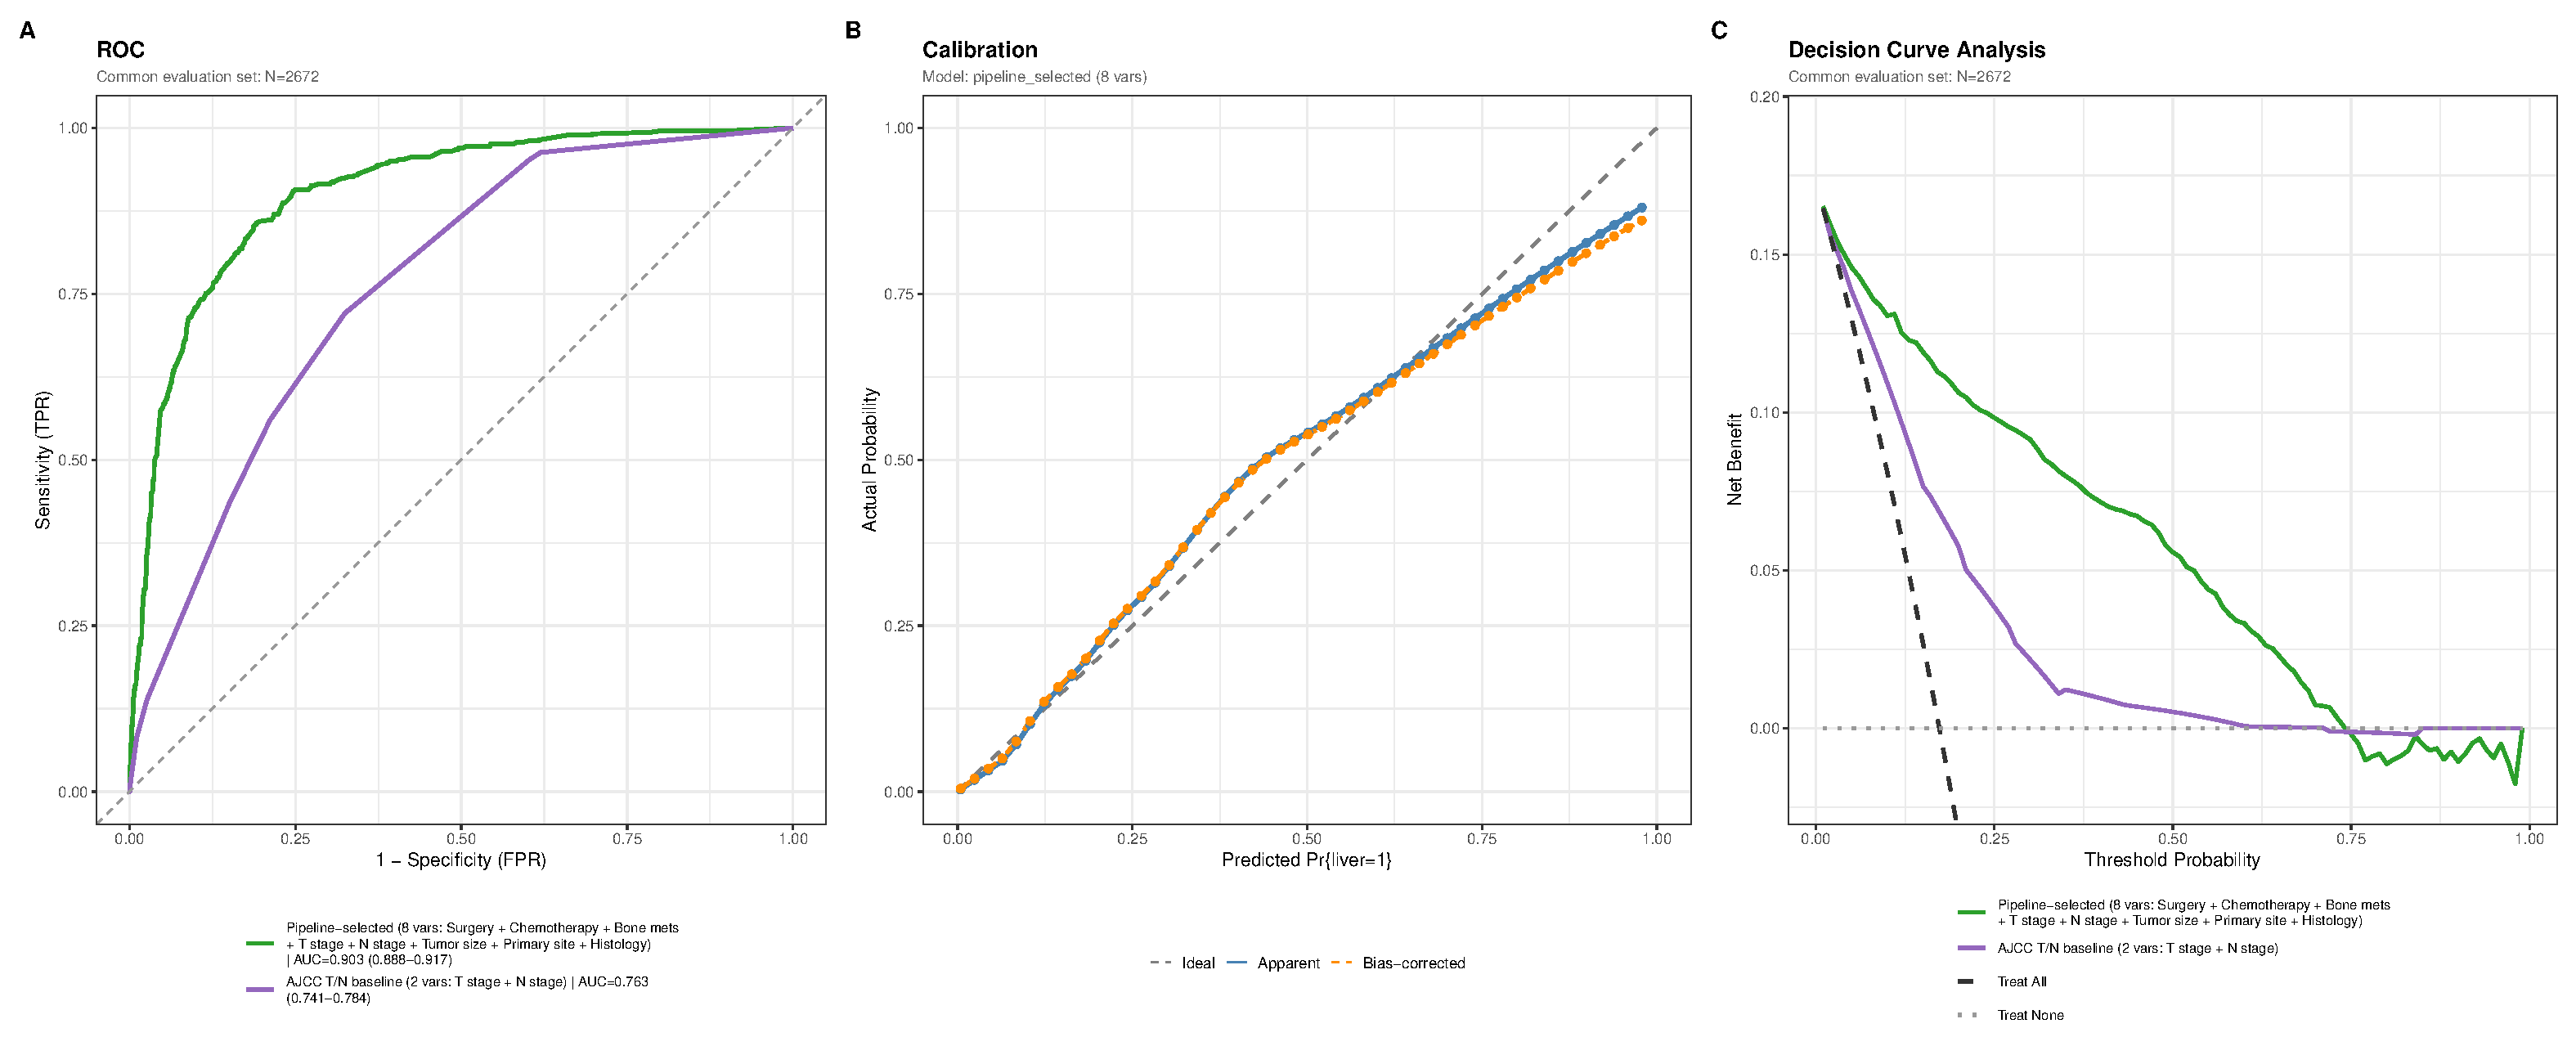
\includegraphics[width=\linewidth]{reference_reproduction/diagnostic_model_evaluation.pdf}
\caption{Diagnostic evaluation of the pipeline-selected 8-variable model in the
complete SEER development cohort. A: ROC curve against the T/N baseline. B:
uncorrected and bootstrap-corrected calibration. C: decision curves against T/N and the
default strategies. The plotted evaluation is not external validation, and the
Brier score discussed in the text belongs to the fixed 5-variable primary
model rather than the plotted pipeline-selected model.}
\label{fig:reference:diagnostic_eval}
\end{figure}
\FloatBarrier

\subsection{Prognostic design and model specifications}
\label{sec:reference:prognostic_methods}

The prognostic analysis starts with 462 patients who had liver metastasis at
diagnosis. Following the reference study, these patients are divided by simple
random sampling into a 70\% training subset and a 30\% internal-validation subset.
The resulting groups contain 323 training records (219 deaths and 104 censored)
and 139 validation records (92 deaths and 47 censored). Because brain metastasis
and some other categories are rare, the split was accepted only when every
categorical predictor required by the primary model was represented in the
training subset. The same patient assignments are used for all prognostic model
development and internal-validation results in this section.

The 12 records with zero recorded survival months are assigned 0.5 months for
model fitting: 11 fall in training and 1 in validation.
This is the implementation's positive-time convention, not a claim that all Cox
estimators require it. The outcome remains death from any cause, with right
censoring for records coded alive.

\begin{table}[htbp]
\centering\small
\caption{Prognostic development split and overall-survival event counts.}
\label{tab:reference:prognostic_split}
\begin{tabular}{@{}lrrr@{}}
\toprule
Cohort & Records & Deaths & Censored \\
\midrule
Training & 323 & 219 & 104 \\
Internal validation & 139 & 92 & 47 \\
\bottomrule
\end{tabular}
\end{table}

The primary Cox specification contains age, grade, histology group, primary
surgery and brain metastasis, following the reference prognostic nomogram
\citep{Li2023}. The training subset contains 2 brain-metastasis records and the
validation subset contains 1. Accordingly, the coefficient is estimable in these
outputs, but very sparsely supported.

Additional models preserve the implementation's alternative selection paths.
Backward Cox/AIC selection retains 9 variables, with bidirectional selection
as a sensitivity procedure. The survival-forest analogue ranks candidates on the
training cohort and evaluates top-$k$ subsets in five folds, selecting 16 variables.
The field labelled \texttt{rmse\_cv} actually contains mean $1-C$, where $C$ is
Harrell's concordance, not root mean squared error. Moreover, the ranking is formed
before those internal folds; this is not nested validation of the complete
ranking-and-selection process. It is used as a selection diagnostic, not as an
unbiased performance estimate.

The union of the Cox/AIC and forest-selected sets, followed by a global
multivariable $p<0.05$ screen, produces the 5-variable data-driven set: age,
histology, grade, N stage and primary surgery. A 6-variable text-screened sensitivity
set and the 2-variable T/N comparator are also retained. These alternatives are
not interchangeable with the primary model; the horizon-specific results below
refer to the primary model and T/N only.

Table~\ref{tab:reference:prognostic_selection} makes the prognostic selection paths
explicit. A total of 4 of the 5 data-driven variables agree with the published nomogram
set. N stage replaces brain metastasis in the data-driven model; the fixed primary
model nevertheless retains brain metastasis so that the paper's stated prognostic
specification is evaluated directly.

\begin{table}[H]
\centering\scriptsize
\caption{Prognostic feature-selection paths and evaluated specifications. All
selection procedures use the 323-record training subset.}
\label{tab:reference:prognostic_selection}
\begin{tabularx}{\linewidth}{@{}p{0.20\linewidth}p{0.25\linewidth}Y@{}}
\toprule
Model or path & Rule and role & Clinical variables retained or specified \\
\midrule
Nomogram-figure primary & Fixed reproduction target from the published prognostic
nomogram & Age, grade, histology, primary surgery and brain metastasis \\
Cox/AIC selection & Backward AIC reduction of the full Cox model & Age, sex, marital
status, histology, grade, T stage, N stage, primary surgery and bone metastasis \\
Survival RF/RFE selection & Pre-ranked random survival forest variables; top-$k$
sets assessed by five-fold mean $1-C$; minimum at $k=16$ & All candidates except
tumour-size group: grade, primary and lymph-node surgery, age, histology,
chemotherapy, N stage, primary site, lung/bone/brain metastasis, race, sex,
radiotherapy, T stage and marital status \\
Pipeline-selected final & Union of Cox/AIC and RF/RFE sets, then global
multivariable $p<0.05$ screen & Age, histology, grade, N stage and primary surgery \\
T/N baseline & Conventional comparator & T stage and N stage \\
\bottomrule
\end{tabularx}
\end{table}

Figure~\ref{fig:reference:prognostic_rfe} shows the survival-forest top-$k$
selection diagnostic using the quantity actually calculated by the implementation.
The minimum mean five-fold error is 0.2629 at 16 variables, compared with 0.2644 at
17 variables. The fold-level variation overlaps substantially, so the selected
$k=16$ should be understood as the numerical minimum of this run rather than
evidence for a uniquely optimal subset.

\begin{figure}[H]
\centering
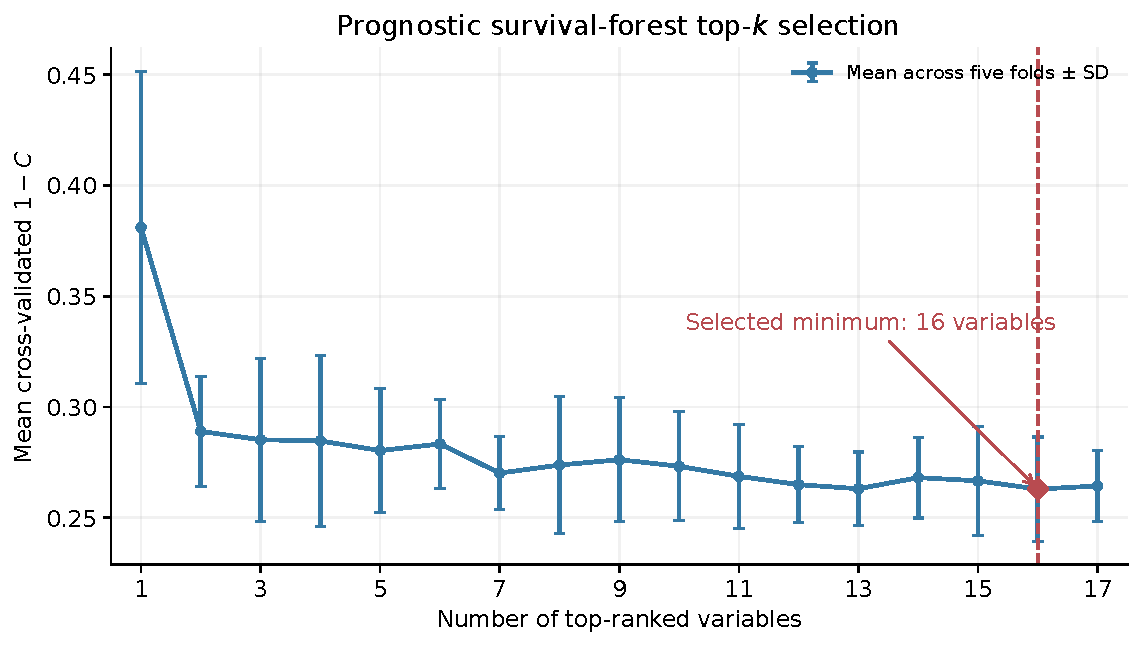
\includegraphics[width=0.88\linewidth]{reference_reproduction/prognostic_rf_rfe_selection.pdf}
\caption{Prognostic survival-forest top-$k$ selection. Points show mean
five-fold $1-C$, where $C$ is Harrell concordance, and error bars show the fold
standard deviation. The vertical line marks the minimum at 16 variables.
The ranking was generated before the folds, so this is not nested validation of
the complete ranking-and-selection procedure.}
\label{fig:reference:prognostic_rfe}
\end{figure}
\FloatBarrier

\paragraph{Evaluation protocol.}
All Cox specifications are fitted on the training subset. Training-set Harrell
C-index is reported for the 6 specifications in
Table~\ref{tab:reference:prognostic_models}; the fixed 5-variable primary Cox
nomogram and T/N baseline are additionally compared by time-dependent ROC/AUC using marginal
inverse probability of censoring weighting (IPCW) at 12, 24 and 36 months in
training and validation. The primary model is also assessed through grouped
survival calibration, horizon-specific decision curves and Kaplan--Meier curves
for risk groups defined by the median training linear predictor. The same risk
threshold is carried unchanged into validation.

\subsection{Prognostic results: association, discrimination and stratification}
\label{sec:reference:prognostic_results}

\paragraph{Comparison of the evaluated Cox specifications.}
Six Cox specifications are retained because they answer different questions. The
5-variable primary model reproduces the prognostic nomogram displayed in the
reference article. The 2-variable T/N model provides a simple clinical baseline
using only tumour and nodal stage. The text-screened sensitivity model uses the
variables named in the article's regression results. The Cox/AIC model applies
backward selection using the Akaike information criterion (AIC), while the random
forest with recursive feature elimination (RF/RFE) model uses a survival forest to
rank predictors and compare progressively smaller subsets. Finally, the
pipeline-selected model combines the variables identified by the Cox/AIC and
RF/RFE procedures and retains those meeting the multivariable selection rule.
Together, these models show how the choice of feature-selection method affects the
result without replacing the prespecified primary model.

Table~\ref{tab:reference:prognostic_models} reports training-set concordance for
all 6 specifications. RF/RFE and Cox/AIC have the largest point estimates (0.758
and 0.757), followed by the 5-variable pipeline-selected model (0.753), the
text-screened sensitivity model (0.743), the primary nomogram model (0.740) and
T/N (0.573). Because model selection and concordance estimation use the same
training subset, these values cannot establish that the more complex models will
perform better in new patients. Horizon-specific internal validation was
prespecified for the primary nomogram and T/N baseline, which form the main
reference-study comparison; the other 4 models are retained to examine how
alternative feature-selection procedures change the training results.

\begin{table}[htbp]
\centering\small
\caption{Training-set performance of the 6 prognostic Cox specifications
($n=323$, 219 deaths). The intervals are Harrell C-index intervals. AIC is
comparable only among models fitted to this same outcome and sample; lower values
indicate better relative fit after accounting for model complexity.}
\label{tab:reference:prognostic_models}
\begin{tabularx}{\linewidth}{@{}Ycrr@{}}
\toprule
Specification & Variables & Harrell C [95\% interval] & AIC \\
\midrule
\csname @@input\endcsname{tables/reference_reproduction/prognostic_model_summary_rows.tex}
\bottomrule
\end{tabularx}
\end{table}

\paragraph{Adjusted associations and model assumptions.}
Table~\ref{tab:reference:cox} gives the primary training-model hazard ratios.
Higher grade, older age and the other-histology group are associated with greater
modelled hazard, while recorded surgery is associated with lower hazard. These
are observational associations conditional on the model covariates. In particular,
the surgery coefficient is not an estimate of a treatment benefit.

\begin{table}[htbp]
\centering\small
\caption{Primary prognostic Cox model: nominal hazard ratios and Wald intervals
from 323 training records and 219 deaths. Interpretations are limited by sparse
brain-metastasis support and evidence against proportional hazards.}
\label{tab:reference:cox}
\begin{tabularx}{\linewidth}{@{}Yrr@{}}
\toprule
Contrast & HR [95\% interval] & Nominal $p$ \\
\midrule
\csname @@input\endcsname{tables/reference_reproduction/prognostic_hr_rows.tex}
\bottomrule
\end{tabularx}
\end{table}

Brain metastasis has HR 2.98 with a wide interval, 0.72--12.40. More importantly,
the Schoenfeld-residual test rejects proportional hazards globally
($p=2.61\times10^{-7}$), with evidence for grade
($p=6.14\times10^{-7}$), histology ($p=0.00156$) and surgery ($p=0.00206$).
This indicates that the associations of these predictors with mortality may
change during follow-up rather than remain constant over time. The corresponding
hazard ratios and survival predictions should therefore be interpreted cautiously,
even when the model separates higher-risk from lower-risk patients well.

\paragraph{Discrimination.}
The primary prognostic model is the fixed 5-variable Cox nomogram containing age,
grade, histology group, primary surgery and brain metastasis. Its training-set
Harrell C-index is 0.7395
(95\% interval 0.7047--0.7744), compared with 0.5728 for T/N. Harrell's C-index
summarises how well each model orders patients by risk across the observed
follow-up. Table~\ref{tab:reference:survival_auc} instead reports discrimination at
12, 24 and 36 months using marginal IPCW to account for censoring. The censoring
weights are estimated separately within the training and validation subsets. The
reported intervals quantify uncertainty in each AUC but do not repeat feature
selection or model fitting.

\begin{table}[htbp]
\centering\small
\caption{Time-dependent AUC [95\% interval] for the fixed 5-variable primary
prognostic Cox model (age, grade, histology group, primary surgery and brain
metastasis) and the 2-variable T/N baseline. Training $n=323$; internal validation
$n=139$. Marginal IPCW and influence-function intervals are used.}
\label{tab:reference:survival_auc}
\begin{tabularx}{\linewidth}{@{}Ycrr@{}}
\toprule
Cohort & Months & Primary Cox model & T/N baseline \\
\midrule
\csname @@input\endcsname{tables/reference_reproduction/prognostic_auc_rows.tex}
\bottomrule
\end{tabularx}
\end{table}

The primary model has higher point estimates than T/N at all three horizons in
both subsets. However, T/N's validation AUCs of 0.391, 0.443 and 0.505 indicate
poor transfer within this one split, not that clinical staging is intrinsically
uninformative. No paired difference test or repeated-split comparison is supplied
by this table. AUC also does not assess the accuracy of absolute survival
probabilities.

Figure~\ref{fig:reference:prognostic_roc} complements the point estimates with the
underlying horizon-specific ROC curves. Panels A--C use the training subset and
Panels D--F use the fixed internal-validation subset; the comparison is restricted
to the fixed 5-variable primary model and the T/N baseline, the 2 specifications
evaluated at each survival horizon.

\paragraph{Calibration and decision curves.}
Survival calibration uses 1,000 bootstrap repetitions in the training subset and
compares grouped predicted survival probabilities with Kaplan--Meier estimates in
the validation subset. The reported slopes and intercepts are calculated by
regressing the observed group-level survival estimates on the corresponding mean
predictions. They are therefore descriptive group-level summaries rather than
standard individual-level calibration measures, and they are not used to claim
that the model is well calibrated in new patients.

The survival decision curves convert predicted survival into mortality risk at
each time horizon and exclude patients censored before that horizon. Because this
calculation does not use IPCW, it provides an approximate view of net benefit and
is not treated as definitive evidence of clinical utility.

\paragraph{Risk-group separation.}
The median training linear predictor, 0.2328 at the reported precision, defines
low- and high-risk groups. The same threshold is applied to validation without
retuning. Median observed survival differs substantially between the groups
(Table~\ref{tab:reference:km}), with log-rank $p<0.001$ in both subsets.
Values smaller than the reported precision are stated as $p<0.001$ rather than
as exact zero. The patient counts, event counts and median survival estimates use
the same risk-group assignments in the table and figure.

\begin{figure}[htbp]
\centering
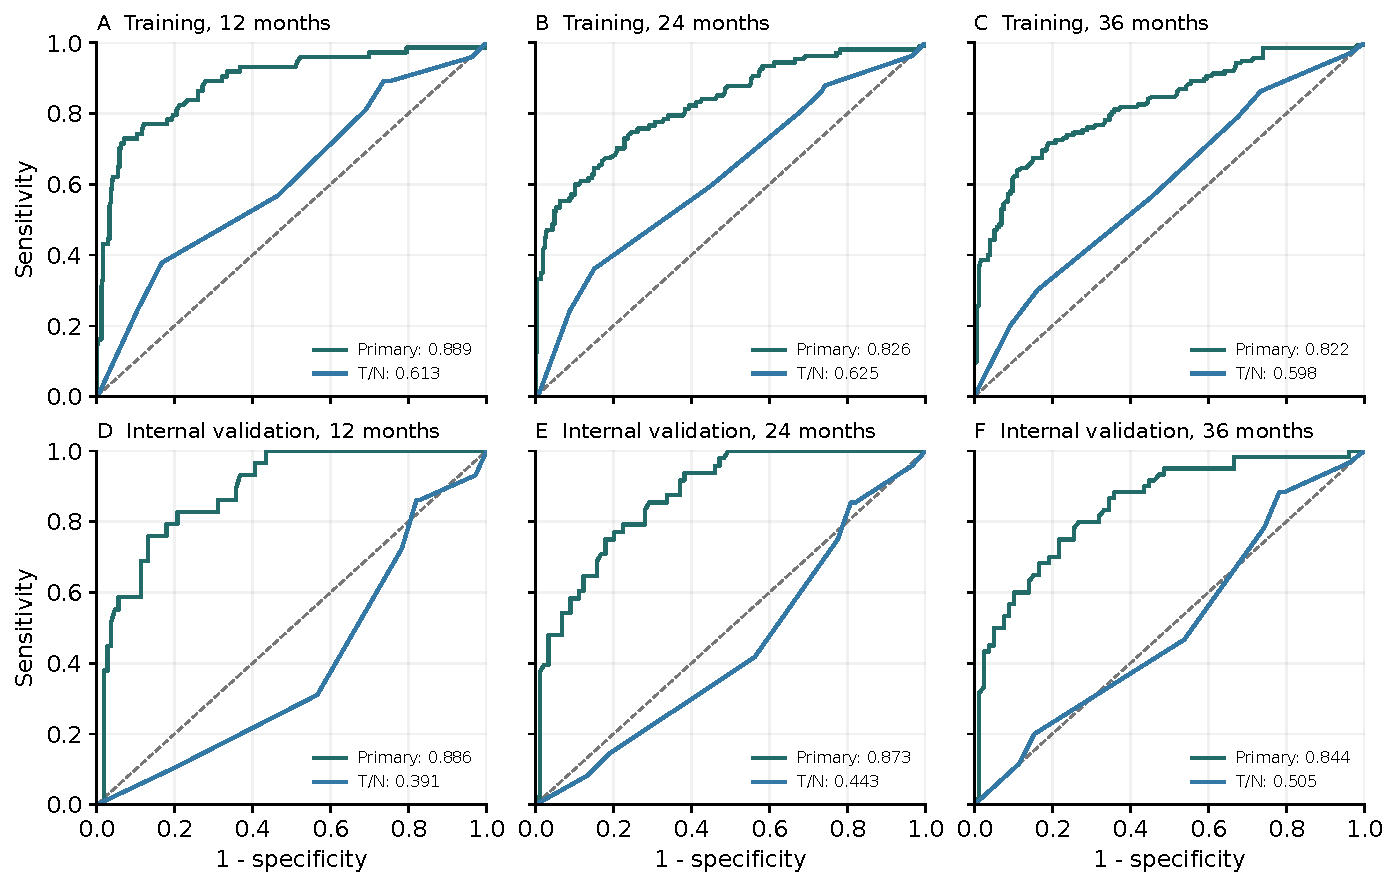
\includegraphics[width=\linewidth]{reference_reproduction/prognostic_time_dependent_roc.pdf}
\caption{Time-dependent ROC curves for the fixed 5-variable primary prognostic
Cox model (age, grade, histology group, primary surgery and brain metastasis) and
the 2-variable T/N baseline at 12, 24 and 36 months. Panels A--C show training
results and Panels D--F show internal-validation results. Marginal IPCW is used;
the results are not estimates from repeated data splits or an external cohort.}
\label{fig:reference:prognostic_roc}
\end{figure}
\FloatBarrier

\begin{table}[H]
\centering\small
\caption{Risk groups from the fixed 5-variable primary prognostic Cox model.
Median overall survival is estimated by Kaplan--Meier, not the median of recorded
follow-up times.}
\label{tab:reference:km}
\begin{tabularx}{\linewidth}{@{}YYrrr@{}}
\toprule
Cohort & Group & Records & Deaths & Median OS (months) \\
\midrule
\csname @@input\endcsname{tables/reference_reproduction/km_summary_rows.tex}
\bottomrule
\end{tabularx}
\end{table}

Table~\ref{tab:reference:km} quantifies the size, number of deaths and median
overall survival of each risk group, while Figure~\ref{fig:reference:km} shows
the full survival trajectories. The curves remain separated through most of the
observed follow-up, although the confidence bands widen at later times as the
number of patients still under observation decreases.

\begin{figure}[H]
\centering
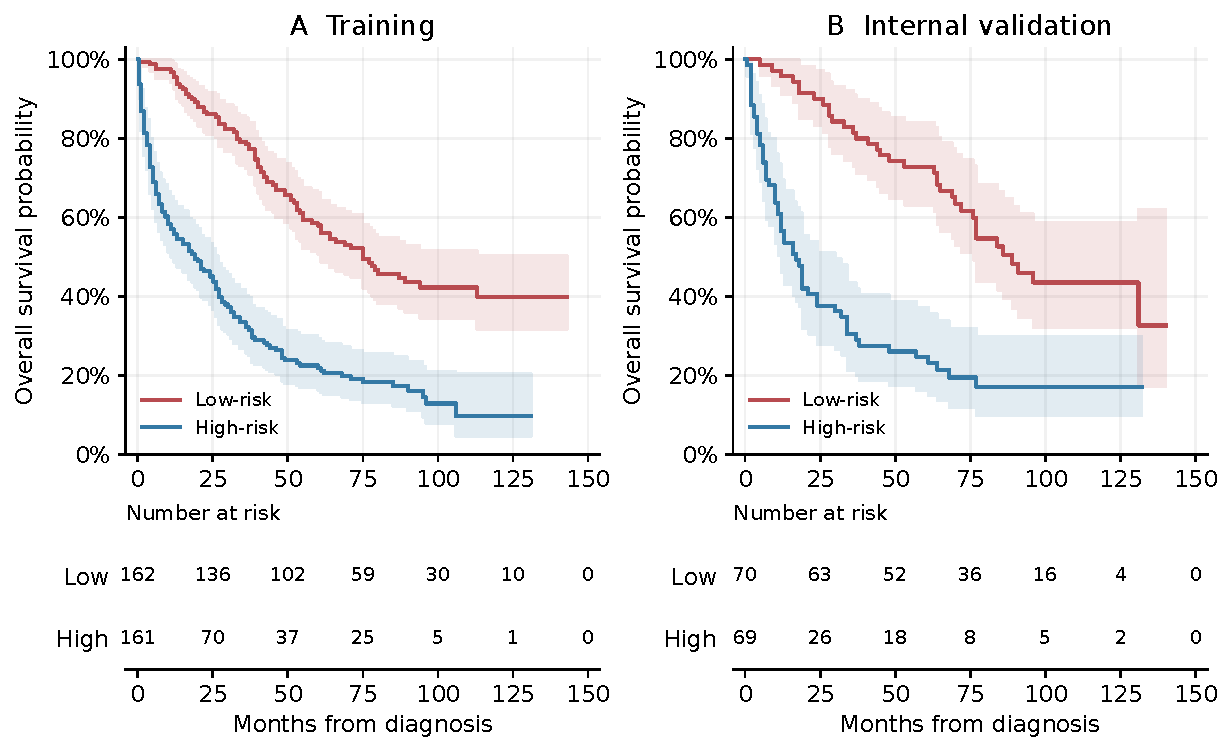
\includegraphics[width=\linewidth]{reference_reproduction/prognostic_km_risk_groups.pdf}
\caption{Overall-survival curves for risk groups defined by the fixed 5-variable
primary prognostic Cox model. Shading denotes
pointwise 95\% log-type Kaplan--Meier intervals; rows below each panel give numbers
at risk. The low/high threshold is learned in training and unchanged in
validation. Sparse late follow-up widens uncertainty. These internally defined
prognostic strata are not independently discovered patient archetypes or external
validation cohorts.}
\label{fig:reference:km}
\end{figure}
\FloatBarrier

\subsection{Focused comparison with the published study}
\label{sec:reference:comparison}

Table~\ref{tab:reference:paper_comparison} summarises the comparisons that are most
informative for this reproduction. For diagnosis, 5 of the paper's 6 stated
risk factors are also in the data-driven model: N stage, primary surgery,
chemotherapy, tumour size and bone metastasis. Grade is selected by LASSO but does
not survive the adjusted screen, whereas T stage, primary site and histology are
additional selected variables. For prognosis, the fixed primary model uses the
same 5 variables as the published nomogram, while the data-driven model shares
age, histology, grade and surgery and substitutes N stage for brain metastasis.

\begin{table}[htbp]
\centering\footnotesize
\caption{Headline discrimination compared with \citet{Li2023}. Published values
are contextual benchmarks, not targets tested on the same patients. Prognostic
AUC triplets are ordered as 1-, 2- and 3-year overall-survival AUC.}
\label{tab:reference:paper_comparison}
\begin{tabularx}{\linewidth}{@{}p{0.14\linewidth}YY@{}}
\toprule
Task & Published study & Present reproduction on the available SEER cohort \\
\midrule
Diagnosis & SEER training-cohort AUC 0.877; external-hospital AUC 0.893. The text identifies
6 variables, while the displayed nomogram omits chemotherapy. & AUC calculated in
the complete SEER development cohort:
0.8795 for the fixed 5-variable nomogram, 0.8947 for the 6-variable text set,
0.9028 for the 8-variable data-driven model, and 0.7628 for T/N. An independent
30-patient external evaluation is reported in Section~\ref{sec:external-validation}. \\
Prognosis & C-index 0.752/0.740/0.760 in training/internal/external cohorts.
Training AUC 0.832/0.794/0.792 and internal AUC 0.832/0.857/0.818. &
training Harrell C-index 0.7395. Primary-model AUC 0.889/0.826/0.822 in training
and 0.886/0.873/0.844 in the single internal-validation subset. \\
\bottomrule
\end{tabularx}
\end{table}
\FloatBarrier

The diagnostic AUCs are numerically close, and the prognostic discrimination is of
the same general magnitude, but neither observation is evidence of equivalence.
The available cohort is larger and comes from a different SEER release; category
frequencies and coding availability changed; the exact feature-selection details
could not always be recovered from the publication; and the paper's external
hospital data were unavailable. Moreover, the diagnostic AUCs were calculated in
the same cohort used to fit the models, so they may overestimate performance in
new patients. The prognostic results come from one 70/30 internal split and may
vary with a different split. These differences prevent a defensible claim that the
present models outperform the published models.

\subsection{Interpretation and transition}
\label{sec:reference:implications}

The reproduction provides conventional logistic- and Cox-regression reference
models for the later experiments, but it does not establish clinical readiness.
The diagnostic analysis shows that the selected predictors depend on the feature-
selection rule, and that permutation and impurity importance can rank the same
variables differently. Treatment variables must also be interpreted cautiously
because their timing and the reasons for receiving treatment are not fully captured
in SEER. In the prognostic analysis, the small number of brain-metastasis cases and
the evidence against constant hazard ratios increase uncertainty. These findings
make calibration, model assumptions and validation in new patients as important as
the discrimination scores.

The primary reference models used in subsequent comparisons are the 5-variable
diagnostic logistic nomogram (grade, N stage, primary surgery, tumour-size group
and bone metastasis) and the 5-variable prognostic Cox nomogram (age, grade,
histology group, primary surgery and brain metastasis). The text-defined,
data-driven and T/N models are retained as comparators so that later analyses can
distinguish a change in representation or model family from a change in the chosen
clinical predictors.

The next section tests these SEER-trained models in the independent UK--Erlangen
cohort. Here, \emph{frozen} means that the fitted coefficients, categorical levels
and decision thresholds are carried over without refitting, feature reselection,
recalibration or threshold adjustment using the external patients. The diagnostic
validation includes the 5-variable primary nomogram, the 6-variable paper-text
model, the 8-variable data-driven model and the T/N baseline. The main prognostic
comparison uses the 5-variable primary Cox model and the T/N baseline, while the
remaining Cox variants are reported as supplementary comparisons. This external
evaluation is performed before the report turns to the TabPFN-based extensions.
